\documentclass[a4paper, 12pt]{article}

\usepackage{cmap}
\usepackage{mathtext} 
\usepackage[T2A]{fontenc}
\usepackage[utf8]{inputenc}
\usepackage[english,russian]{babel}	

\usepackage{amsfonts,amssymb,amsthm,mathtools}
\usepackage{amsmath}
\usepackage{icomma} 

\usepackage{graphicx} 
\graphicspath{{Picturies/}}
\usepackage{wrapfig}

\usepackage{array,tabularx,tabulary,booktabs}
\usepackage{longtable}
\usepackage{multirow}

\usepackage{caption}
\captionsetup{labelsep=period}

\renewcommand{\phi}{\varphi}
\newcommand{\eps}{\varepsilon}
\renewcommand{\AA}{\ensuremath{\mathring{A}}}
\newcommand{\parag}[1]{\paragraph*{#1:}}

\newcounter{Points}
\setcounter{Points}{1}
\newcommand{\point}{\arabic{Points}. \addtocounter{Points}{1}}

\author{Вязовцев Андрей, Б01-005}
\date{05.10.22}
\title{Лабораторная работа 5.4.2. Исследование энергетического спектра $\beta$-частиц и определение их максимальной энергии при помощи магнитного спектрометра.}

\begin {document}

\maketitle

\parag {Цель работы} С помощью магнитного спетрометра исследовать энергетический спектр $\beta$-частиц при распаде ядер $~^{137}$Cs и определяется их максимальная энергия.

\parag {В работе используются} магнитный спектрометр с короткой линзой.

\parag {Теоретическая справка} ~\\

Явление радиоктивности состоит в самопроизвольном распаде ядер с испусканием одной или нескольких частиц. К числу радиоактивных процессов относятся $\alpha$- и $\beta$-распады (в том числе и $K$-захват), $\gamma$-излучение, деление ядер, а также испускание запаздывающих нейтронов и протонов. В нашей работе мы будем рассматривать второе явление.

Бета-распад --- процесс самопроизвольного превращения нестабильного ядра в ядро-изобар (ядро с тем же числом нуклонов, т.~е. с одинаковым массовым числом $A$) с зарядом, отличным от исходного на $\Delta Z = \pm 1$ за счёт испускания электрона (позитрона) или захвата электрона с атомной оболочки. Главной особенностью $\beta$-распада является то, что он обусловлен не ядерными и не электромагнитными силами, а слабым взаимодействием. Период полураспада изменяется от ничтожных долей секунды до $10^{18}$ лет, а энегрия от $18$ кэВ до $13.4$ МэВ.

В данной работе мы будем иметь дело с электронным распадом:

\[
    ~^A_Z X \rightarrow ~^A_{Z+1} X + e^- + \tilde{\nu}
\]

Вероятность $d\omega$ того, что при распаде электрон вылетит с импульсом $d^3\vec{p}$, а антинейтрино с импульсом в интервале $d^3\vec{k}$ равна

\begin{equation}
    d\omega = D \delta (E_e - E - ck) d^3p d^3p
\end{equation}

где $E_e$ --- максимальная энергия электрона, $E$ --- его кинетическая энегрия, $D$ --- некоторый коэффициент пропорциональности, при этом:

\begin{equation}
    E_e - E - ck = 0
\end{equation}

Соответственно, для электрона с импульсом $[p, ~p+dp]$ и антинейтрино с импульсом $[k, ~k+dk]$ количество распадов $dN$ на $N_0$ частиц определяется выражением:

\begin{equation}
    dN = N_0 d\omega
\end{equation}

В нерелятевистком приближении (наш случай) можено получить, что:

\begin{equation}
    \frac{dN}{dE} \approx \sqrt{E} (E_e - E)^2
\end{equation}

Дочерние ядра, возникающие в результате $\beta$-распада, нередко оказываются возбуждёнными. Возбуждённые ядра отдают свою энергию либо излучая $\gamma$-квант, либо передавая избыток энергии одному из электронов с внутренних оболочек атома. Излучаемые в таком процессе электроны имеют строго определённую энергию и называются конверсионными.

\parag {Экспериментальная установка} ~

Энергию $\beta$-частиц определяют с помощью $\beta$-спектрометров. В работе используется магнитный спектрометр с <<короткой линзой>>. На рис. \ref{img:work1} изображена схема установки. А на рис. \ref{img:work2} --- общая блок-схема.

Как показывает расчёт, для заряженных частиц тонкая катушка эквивалента линзе. Для фокусного расстояния $f$, силы тока $I$ и импульса электрона $p$ верно:

\[
    \frac{1}{f} \propto \frac{I^2}{p^2}
\]

Отсюда следует:

\begin{equation}
    p = k I
    \label{eq:coef}
\end{equation}

\begin{figure}[!h]
    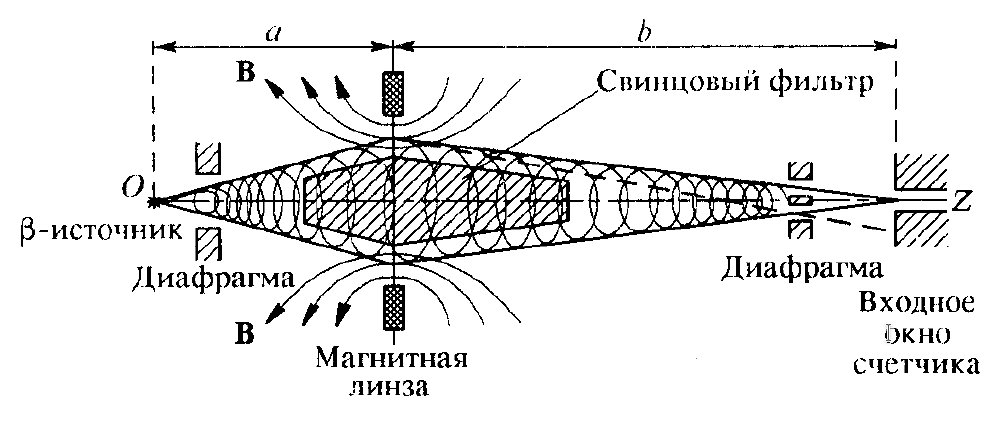
\includegraphics[scale = 0.4]{Workplace1}
    \centering
    \caption{Схема $\beta$-спектрометра с короткой магнитной линзой}
    \label{img:work1}
\end{figure}

\begin{figure}[!h]
    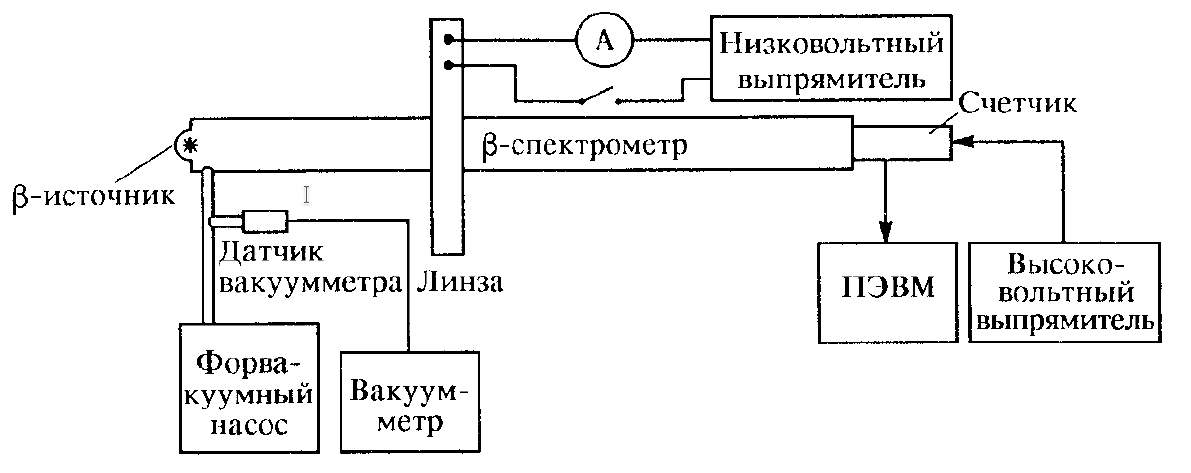
\includegraphics[scale = 0.4]{Workplace2}
    \centering
    \caption{Блок-схема установки для изучения $\beta$-спектра}
    \label{img:work2}
\end{figure}

\parag {Ход работы} ~\\

\point Включим пересчётный прибор, высоковольтный выпрямитель и вакуумметр и дадим им прогреться 10-15 минут. Насосом сделаем, чтобы давление в спектрометре было не больше $0.1$ Тор. Насос отключим, соединив его с атмосферой.

\point Установим рабочее напряжение на ФЭУ. Убедимся, что $\beta$-спектрометр правильно работает.

\point Проведём измерения, особое внимание уделим конверсионному пику. Каждое будем проводить в течение $100$ секунд. Результаты представлены в таблице \ref{tab:meas}.

\begin{table}[!h]
    \centering
    \begin{tabular}{|c|c|c|c|c|c|c|c|c|c|c|}
        \hline
        $I$, А & 0.2 & 0.4 & 0.6 & 0.8 & 1.0 & 1.1 & 1.2 & 1.3 & 1.4 & 1.5 \\ \hline
        $N, ~\frac{1}{с}$ & 1.36 & 1.61 & 2.03 & 2.07 & 2.70 & 3.44 & 3.73 & 4.68 & 5.20 & 5.83 \\ \hline
    \end{tabular}
    \\~\\
    \begin{tabular}{|c|c|c|c|c|c|c|c|c|c|c|}
        \hline
        $I$, А & 1.6 & 1.7 & 1.8 & 1.9 & 2.0 & 2.1 & 2.2 & 2.3 & 2.4 & 2.5 \\ \hline
        $N, ~\frac{1}{с}$ & 6.41 & 6.93 & 8.21 & 8.23 & 7.88 & 8.09 & 7.35 & 6.70 & 6.62 & 5.56 \\ \hline
    \end{tabular}
    \\~\\
    \begin{tabular}{|c|c|c|c|c|c|c|c|c|c|}
        \hline
        $I$, А & 2.6 & 2.7 & 2.8 & 2.9 & 3.0 & 3.05 & 3.1 & 3.15 & 3.2 \\ \hline
        $N, ~\frac{1}{с}$ & 4.39 & 3.49 & 3.30 & 3.68 & 5.17 & 7.27 & 9.66 & 12.41 & 12.63 \\ \hline
    \end{tabular}
    \\~\\
    \begin{tabular}{|c|c|c|c|c|c|c|c|c|c|}
        \hline
        $I$, А & 3.3 & 3.35 & 3.4 & 3.45 & 3.5 & 3.6 & 3.7 & 3.9 & 4.1 \\ \hline
        $N, ~\frac{1}{с}$ & 12.04 & 11.05 & 8.74 & 6.52 & 4.47 & 2.62 & 1.42 & 0.73 & 0.62 \\ \hline
    \end{tabular}
    \caption {Измерения на $\beta$-спектрометре}
    \label{tab:meas}
\end{table}

\point Измерим фон. Результаты --- в таблице \ref{tab:back}.

\begin{table}[!h]
    \centering
    \begin{tabular}{|c|c|c|}
        \hline
        $t$, с & 300 & 300\\ \hline
        $N, ~\frac{1}{с}$ & 1.3593 & 0.5964\\ \hline
        $I$, А & 0 & 4.25 \\ \hline
    \end{tabular}
    \caption {Фон спектрометра}
    \label{tab:back}
\end{table}

\newpage

\parag {Обработка результатов} ~\\

\point Вычтем из измерений фон и построим график $N (I)$. При этом уровень конверсионного пика приблизим распределением Гаусса, а другую часть графика --- уравнением вида:

\[
    N(I) = a \cdot \sqrt{I} (I - b)^2 + c
\]

\begin{figure}[!h]
    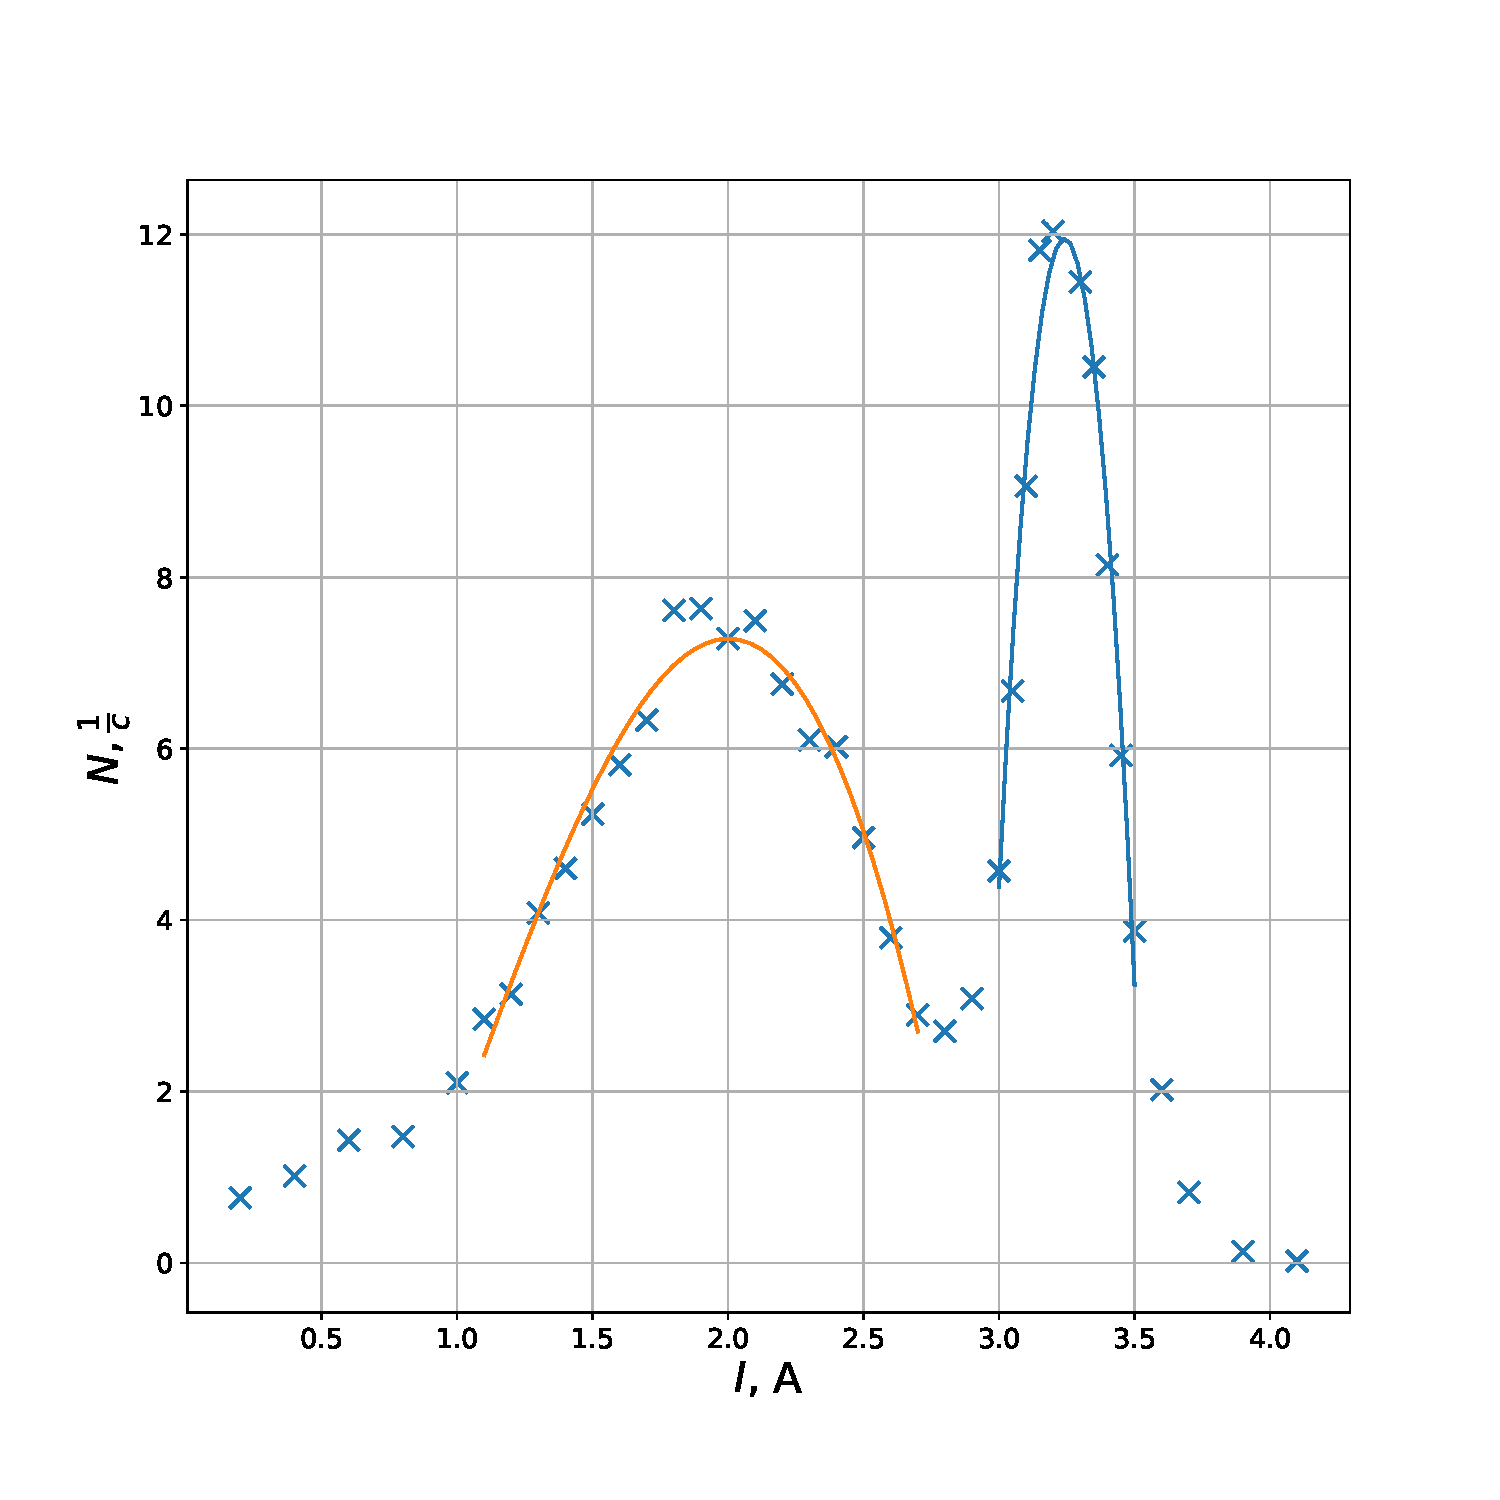
\includegraphics[scale = 0.4]{N_I}
    \centering
    \caption{Главный график}
    \label{img:N_I}
\end{figure}

\point Найдём константу прибора по энергии электронов внутренней конверсии $~^{137}Cs$, равной $T_к = 624$ кЭв. Т.~к. $m = 511$ кэВ, то $E_к = 1135$ кэВ и $p_к = 1013$ кэВ. Т.к. $I = (3.241 \pm 0.004)$ А, то 

\[
    k = (312.7 \pm 0.4) ~\frac{кэВ}{А}
\]

\point Построим график Ферми-Кюри. Из графика получаем, что:

\[
    E_max = (1140 \pm 30) кэВ
\]

\begin{figure}[!h]
    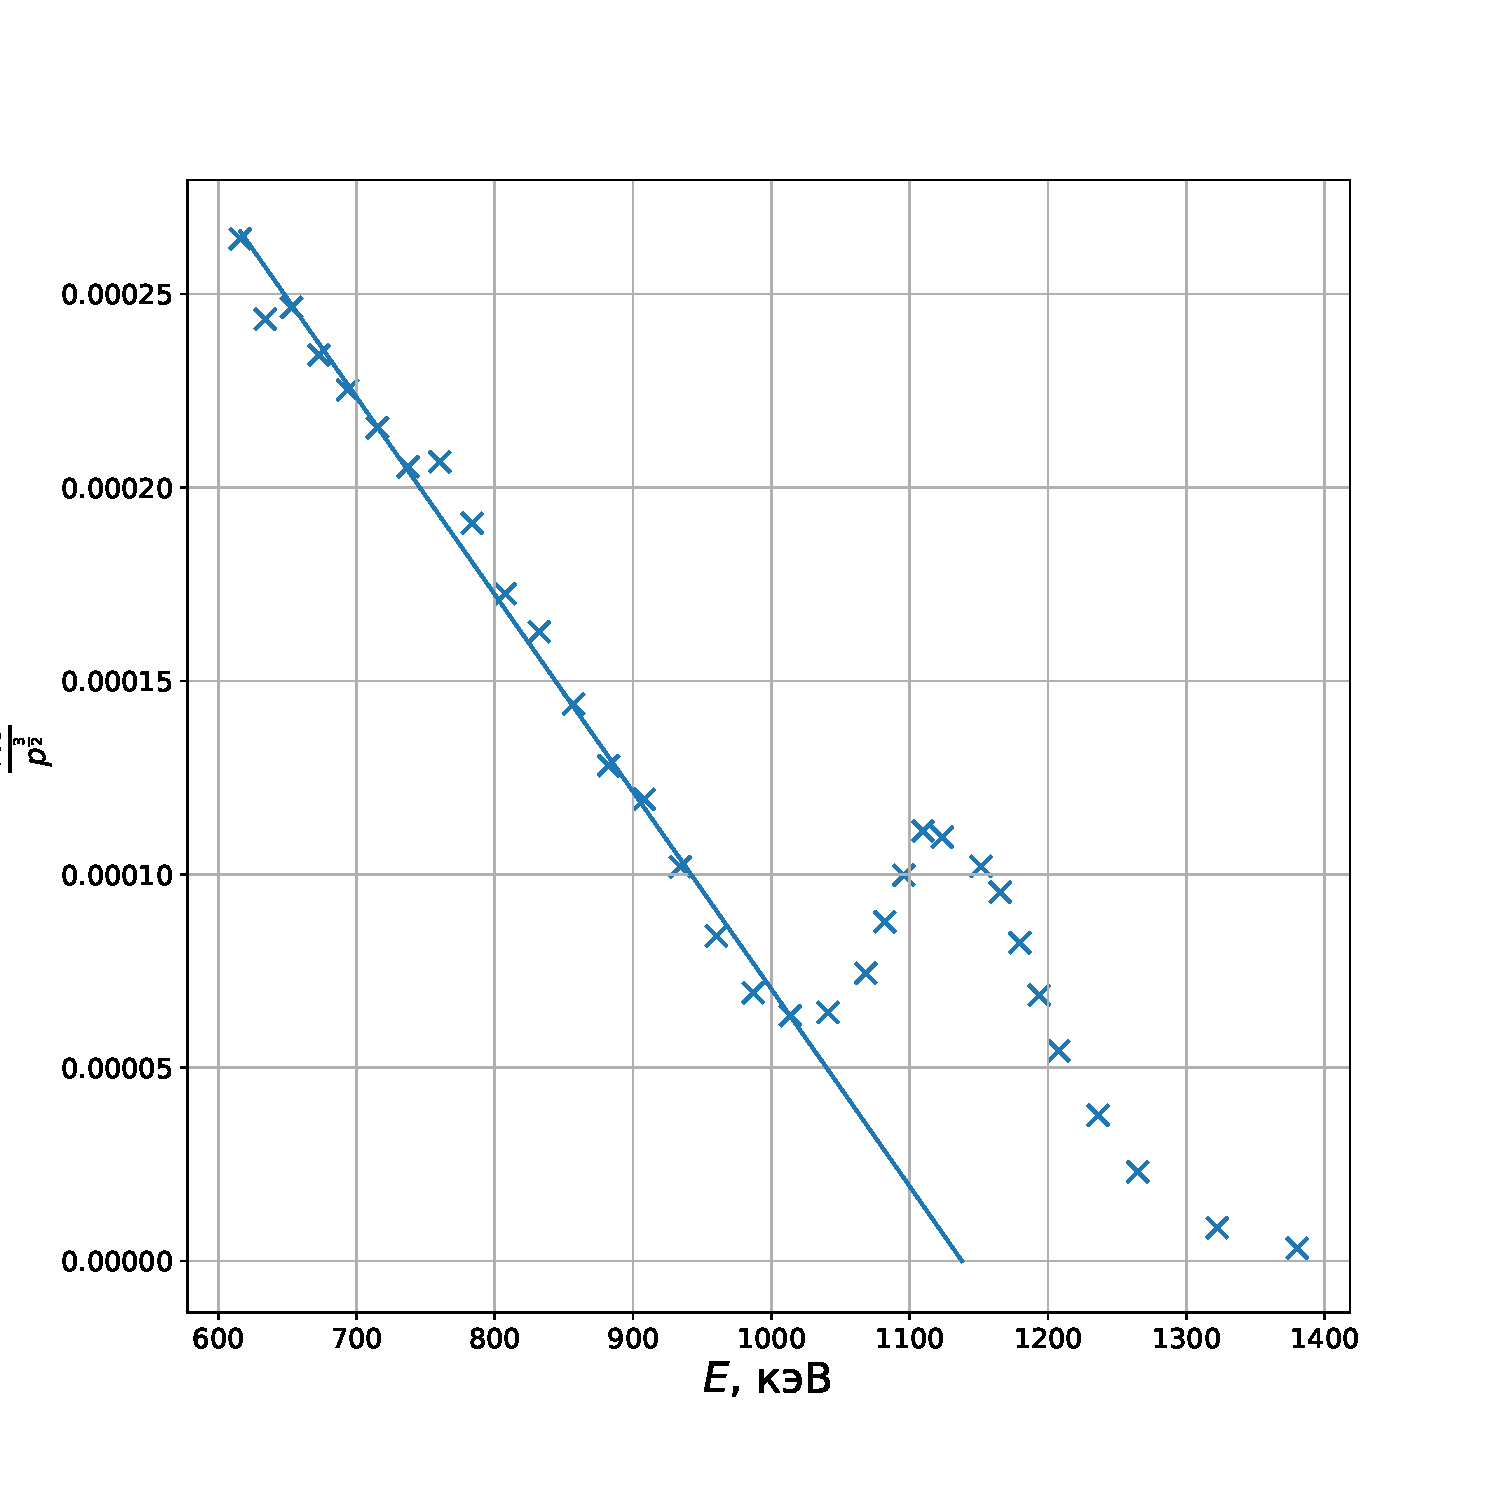
\includegraphics[scale = 0.4]{F-K}
    \centering
    \caption{График Ферми-Кюри}
    \label{img:F_K}
\end{figure}

\end {document}
